\documentclass[a4paper]{article}

\usepackage[english]{babel}
\usepackage[utf8]{inputenc}
\usepackage{amsmath}
\usepackage{graphicx}
\usepackage{epsfig}
\usepackage[colorinlistoftodos]{todonotes}
\usepackage[hidelinks]{hyperref}
\usepackage[margin=1.3in]{geometry}
\usepackage{booktabs}
\usepackage{caption}
\usepackage{subcaption}
\usepackage{longtable}


\title{A Replication of 'Annual Report Readability, Current Earnings, and Earnings Persistence'}

\author{Wenqian Chen}
\setlength{\parskip}{1em}     
\setlength{\parindent}{0em}   

\date{April 2025}

\newcommand{\gfigure}[4]
{
	\begin{figure}
      \begin{center}
          \includegraphics[#3]{#4}
          \caption{#1}
          \label{Figure:#2}
      \end{center}
    \end{figure}
}
\newcommand{\figref}[1]{Figure~\ref{Figure:#1}}

\begin{document}
\maketitle

\begin{abstract}
This study examines the association between the readability of annual reports and firm performance and earnings persistence, for 10-K filings during the period 2016–2021. Following Li.(2008), I use the Fog Index and document length to measure textual readability and additionally incorporate the Bog Index metrics introduced by Bonsall et al (2017) to complement the analysis. The replication results, which are also reflected through evidence of a negative association between readability and earnings persistence, indicate that firms may use less readable disclosures to present less persistent good news. These findings are consistent with prior literature and underscore the value of textual analysis in enhancing the informativeness of financial disclosures.

\end{abstract}

\section{Introduction}

Financial information plays a critical role in shaping investor perceptions and informing equity valuation. Investors rely heavily on publicly available disclosures such as 10-K filings, conference call transcripts, and analyst reports to evaluate the potential future prospects of a company. Recent research increasingly applies textual analysis to extract informative signals from these narratives, enabling researchers to better understand the strategic communication behaviors of firms. Approaches ranging from pre-defined word categorizations to advanced machine learning algorithms are used to evaluate disclosure tone, complexity, and indicators of managerial obfuscation, misreporting, or potential fraud. These analytical methods help uncover how disclosure strategies relate to underlying firm fundamentals, impacting investor decisions and market efficiency.\par

This paper replicates the well-cited readability study in accounting by Li(2008)\cite{li2008annual}, published in the Journal of Accounting and Economics. Unlike the earlier paper’s example, which focused on 10-K filed between 1994 and 2004, this replication examines a more recent sample of 10-K filings during the period 2016–2021, resulting in 18,626 firm-year observations. Given the critiques of Loughran and McDonald (2014)\cite{loughran2014measuring}, who argue that traditional readability measures such as the Fog Index may perform poorly in financial materials because some 'complex' words can be easily understood in a financial context, this study employs the Bog Index introduced by Bonsall et al. (2017)\cite{bonsall2017plain}. Unlike the Fog Index, which simplistically classifies word complexity based on syllable counts, the Bog Index captures multiple SEC-recommended plain English attributes and has been validated empirically through controlled experiments and regulatory interventions (Bonsall et al., 2017). Thus, it provides a more nuanced measure of readability in financial disclosures.\par

The rest of this study is organized as follows: Section 2 outlines the readability measures, Section 3 elaborates on the data, Section 4 presents the empirical findings, and Section 5 concludes the article.


\section{Readability Measures}

Following Li (2008), I employ two commonly used textual metrics to assess the readability of annual reports: the Fog Index and document length. In addition, I use the Bog Index introduced by Bonsall et al. (2017) as a supplemental measure to address limitations associated with traditional readability proxies.

\textbf{Fog Index.} The Fog Index, introduced by Gunning (1952), is one of the most widely used readability measures in accounting and finance research. It is calculated as follows:
\[
\text{Fog Index} = 0.4 \left( \frac{\text{Words}}{\text{Sentences}} + 100 \times \frac{\text{Complex Words}}{\text{Words}} \right),
\]
where complex words are defined as those containing three or more syllables. A higher Fog score indicates greater textual complexity. Consistent with prior literature, scores above 18 are typically considered unreadable, 14–18 difficult, 12–14 ideal, 10–12 acceptable, and below 10 overly simplistic.

\textbf{Length.} The second measure is the length of the annual report, calculated as the natural logarithm of the total number of words:
\[
\text{Length} = \log(\text{NWords}),
\]
where $\text{NWords}$ denotes the word count of the document. Longer reports may increase information processing costs for investors. The log transformation reduces skewness due to outliers in word counts across firms and years.

\textbf{Bog Index.} To complement the above measures, I include the Bog Index, which uses a broader set of plain English attributes recommended by the SEC (1998). It is calculated as:
\[
\text{Bog Index} = \text{Sentence Bog} + \text{Word Bog} - \text{Pep},
\]
where \textit{Sentence Bog} penalizes long or convoluted sentence structures, \textit{Word Bog} captures lexical complexity and violations of plain English (e.g., use of passive voice or legal jargon), and \textit{Pep} rewards clarity-enhancing features such as sentence variety and familiar vocabulary. Higher values indicate lower readability.

I compute the Fog Index and document length using the \texttt{py-readability-metrics} package in Python. Bog Index scores are obtained from the authors’ website associated with Bonsall et al. (2017), which are generated using the StyleWriter software. All readability measures are constructed at the firm-year level based on the full 10-K text and the MD\&A section.


\section{Sample and data description}
\subsection{Sample}
This study analyzes 10-K filings for CRSP-COMPUSTAT firm-years from 2016 to 2021, primarily covering fiscal years 2015–2020 due to the December fiscal year-end convention. Following Li (2008), I apply the similar sample construction procedure, including CRSP-COMPUSTAT matching, CIK linking, 10-K retrieval from EDGAR, text processing, and exclusion based on extreme operating earnings. Readability are computed from the cleaned narrative text. 

\subsection{Summary statistics}

\begin{table}[ht]
\centering
\caption{Summary statistics}  
\label{tab:summary_statistics}
\begin{tabular}{lcccccc}
  \hline
 & Mean & Median & Std. Dev & 25th & 75th & N \\ 
  \hline
  \midrule
  \\[0.5ex]
Year & - & 2019 & - & 2017 & 2020 & 18626 \\ 
  Earnings & -0.02 & 0.03 & 0.21 & -0.03 & 0.09 & 18626 \\ 
  Market-to-book & 1.09 & 0.44 & 2.52 & -0.28 & 1.56 & 18423 \\ 
  Market value of equity (\$MM) & 8939.62 & 855.59 & 49300.66 & 188.10 & 3671.22 & 18453 \\ 
  Book value of assets (\$MM) & 12919.07 & 1055.87 & 91181.62 & 213.25 & 4312.00 & 18626 \\ 
  \midrule
\\[0.5ex]
\multicolumn{7}{l}{\textit{Whole annual report}}\\[0.5ex]
  Fog & 20.94 & 20.87 & 1.33 & 20.14 & 21.61 & 18626 \\ 
  Fog$_{t}$ - Fog$_{t-1}$ & 0.08 & 0.06 & 1.20 & -0.22 & 0.38 & 14237 \\ 
  Length & 11.04 & 11.02 & 0.46 & 10.76 & 11.30 & 18626 \\ 
  Length$_{t}$ - length$_{t-1}$ & -0.01 & -0.00 & 0.34 & -0.13 & 0.11 & 14237 \\ 
  Bog & 90.88 & 90.00 & 9.32 & 85.00 & 96.00 & 18626 \\
  Bog$_{t}$ - Bog$_{t-1}$ & 1.51 & 1.00 & 5.56 & -1.00 & 3.00 & 14237 \\ 
    \midrule
\\[0.5ex]  
\multicolumn{7}{l}{\textit{MD\&A section}}\\[0.5ex]
  Fog & 19.93 & 20.01 & 1.89 & 19.02 & 21.00 & 16953 \\ 
  Fog$_{t}$ - Fog$_{t-1}$ & 0.13 & 0.06 & 1.21 & -0.22 & 0.40 & 12530 \\ 
  Length & 8.37 & 9.13 & 2.20 & 8.58 & 9.48 & 18626 \\ 
  Length$_{t}$ - length$_{t-1}$ & -0.08 & 0.00 & 2.00 & -0.10 & 0.08 & 14237 \\ 
   \hline
\end{tabular}
\end{table}

Table 1 presents summary statistics for the readability. The mean Fog index is 20.94 (median 20.87), which exceeds the threshold of 18 typically associated with unreadable text. The mean (median) length is 11.04 (11.02), and the mean Bog index is 90.88 (90.00). These figures are consistent with prior studies indicating that annual reports often employ overly complex language (e.g., Li, 2008; Bonsall et al., 2017). The standard deviation of the Fog index (1.33) and report length (0.46) indicates substantial cross-sectional variation. Similarly, year-over-year changes in Fog ($\mathrm{SD} = 1.20$) and length ($\mathrm{SD} = 0.34$) suggest notable temporal variation.

The MD\&A section is comparatively more readable, with a lower mean Fog score (19.93) than the full report, indicating reduced linguistic complexity. Notably, the readability of the MD\&A section exhibits greater cross-sectional variation ($\mathrm{SD} = 1.89$)than that of the full report, and MD\&A length is also more variable ($\mathrm{SD} = 2.20$). Additionally, Year-over-year changes in MD\&A Fog ($\mathrm{SD} = 1.21$)  and length ($\mathrm{SD} = 2.00$) further underscore substantial temporal variation in narrative disclosures.

Figures 1 and 2 illustrate readability trends for the full 10-K and the MD&A section from 2016 to 2021. Over this period, the median Fog and Bog indices both increase steadily, suggesting that annual reports have become increasingly difficult to read. The continued rise in Bog scores, in particular, indicates a decline in adherence to plain English writing conventions. By contrast, the length of annual reports(measured as the logarithm of word count) has declined since 2019 for both the full report and the MD&A section. This shift aligns with the SEC’s 2018 adoption of the Inline XBRL mandate, which allows filers to submit a single integrated human- and machine-readable document, potentially encouraging more concise reporting.

\begin{figure}[htbp] 
    \centering
    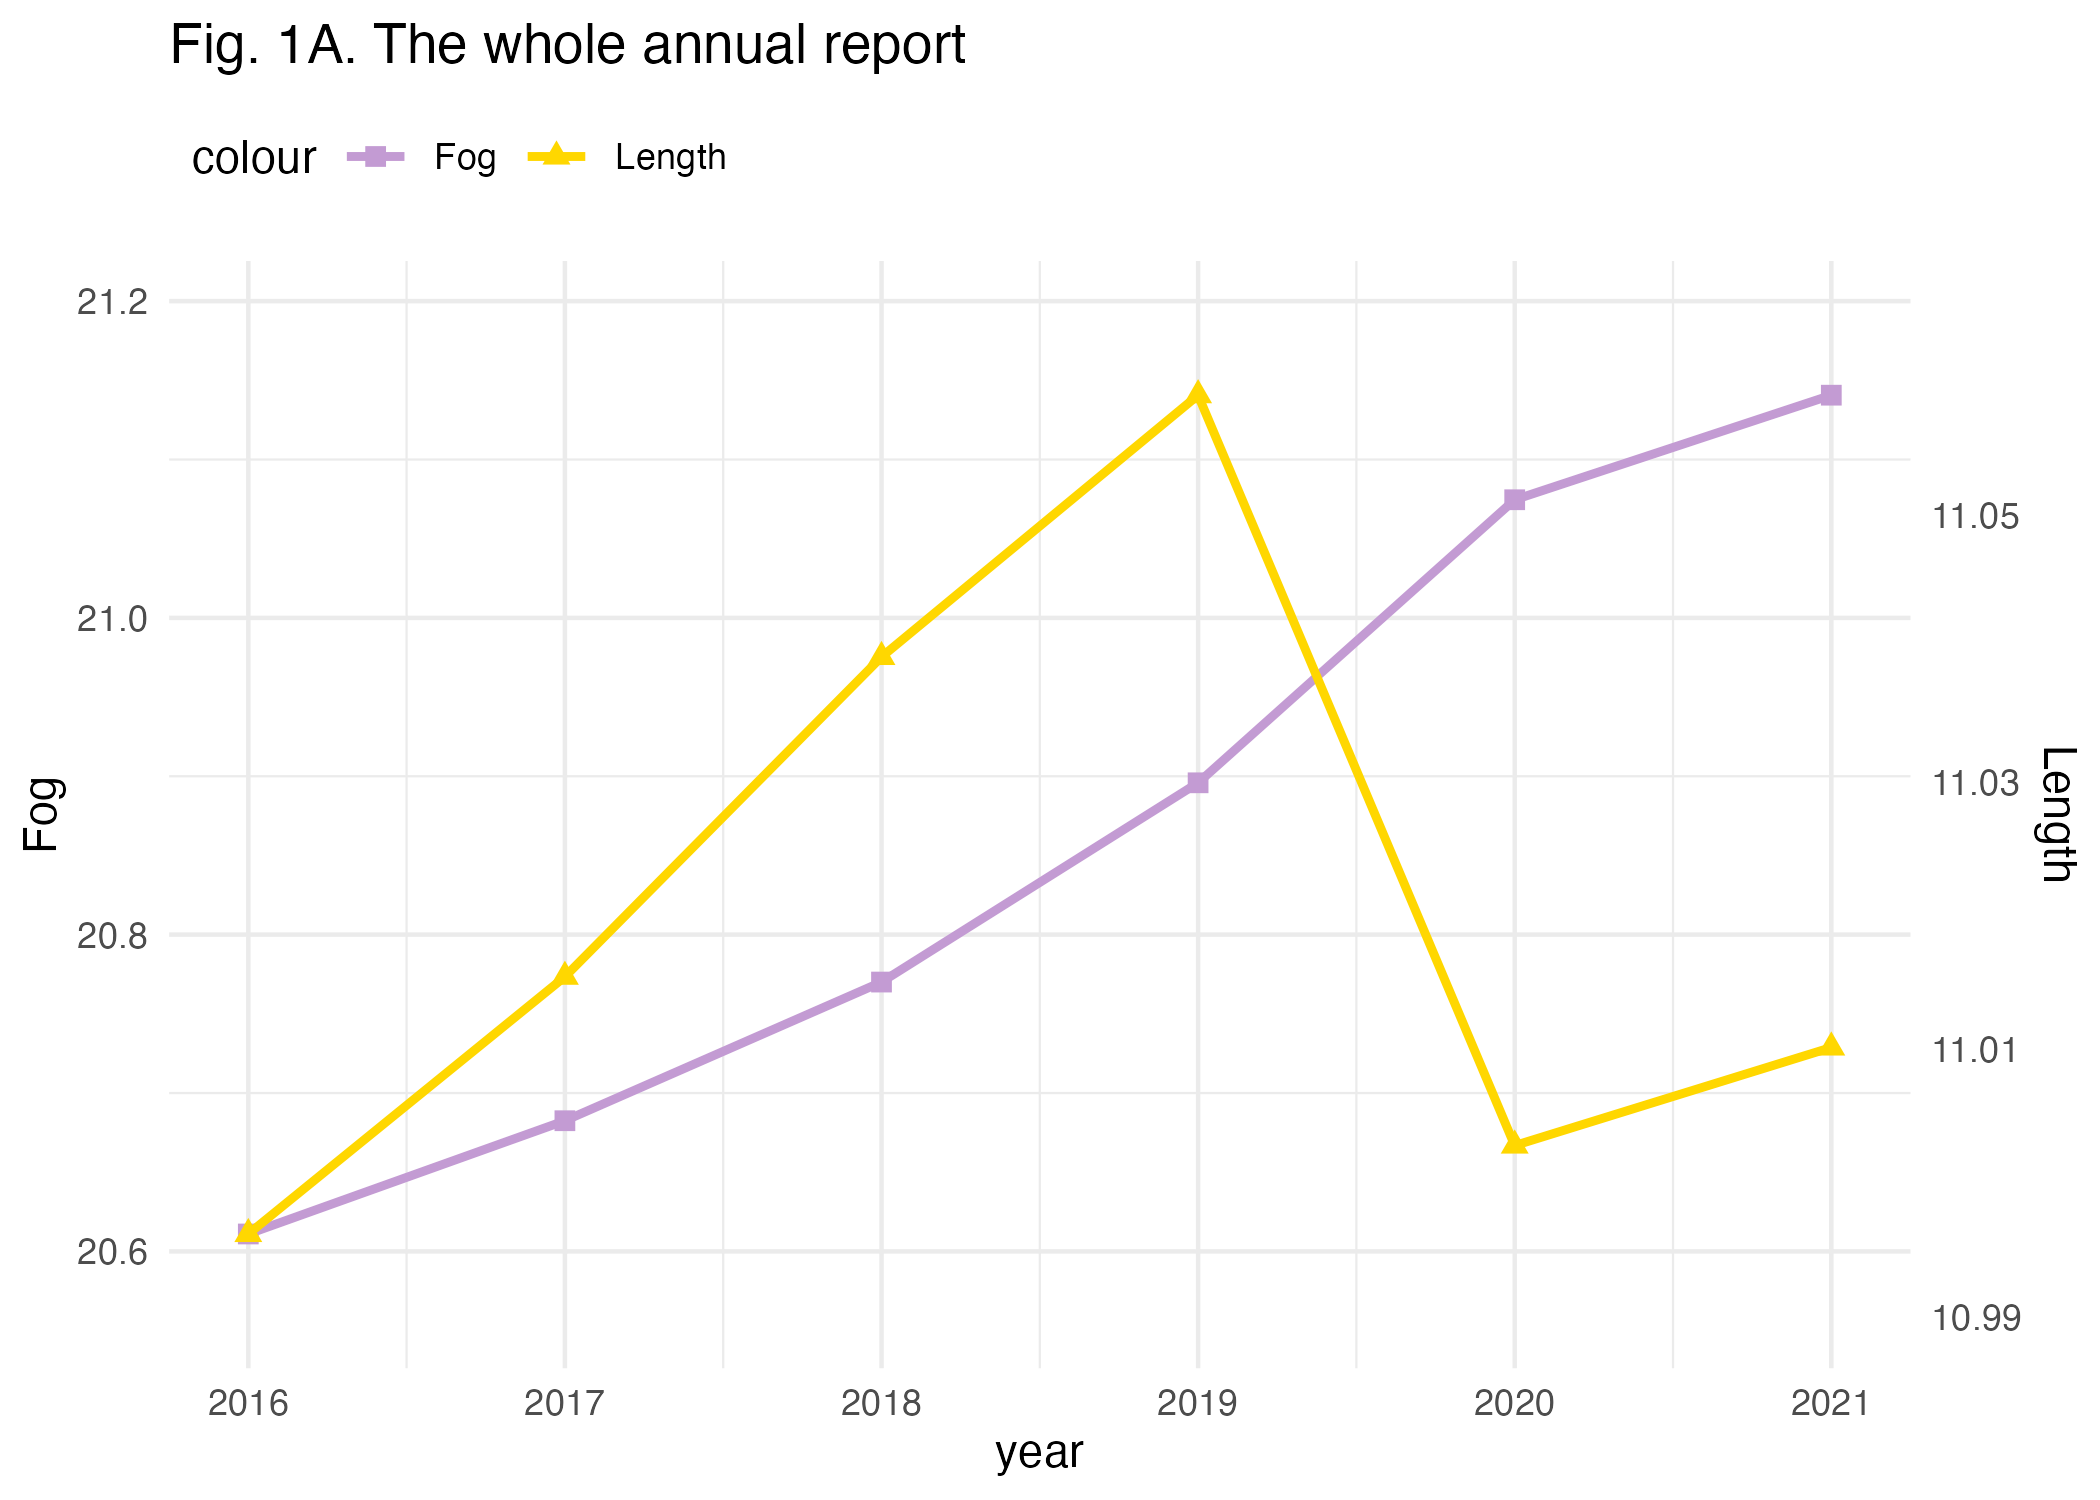
\includegraphics[width=\linewidth]{Images/fig1a.png}
\end{figure}

\begin{figure}[htbp]
    \centering
    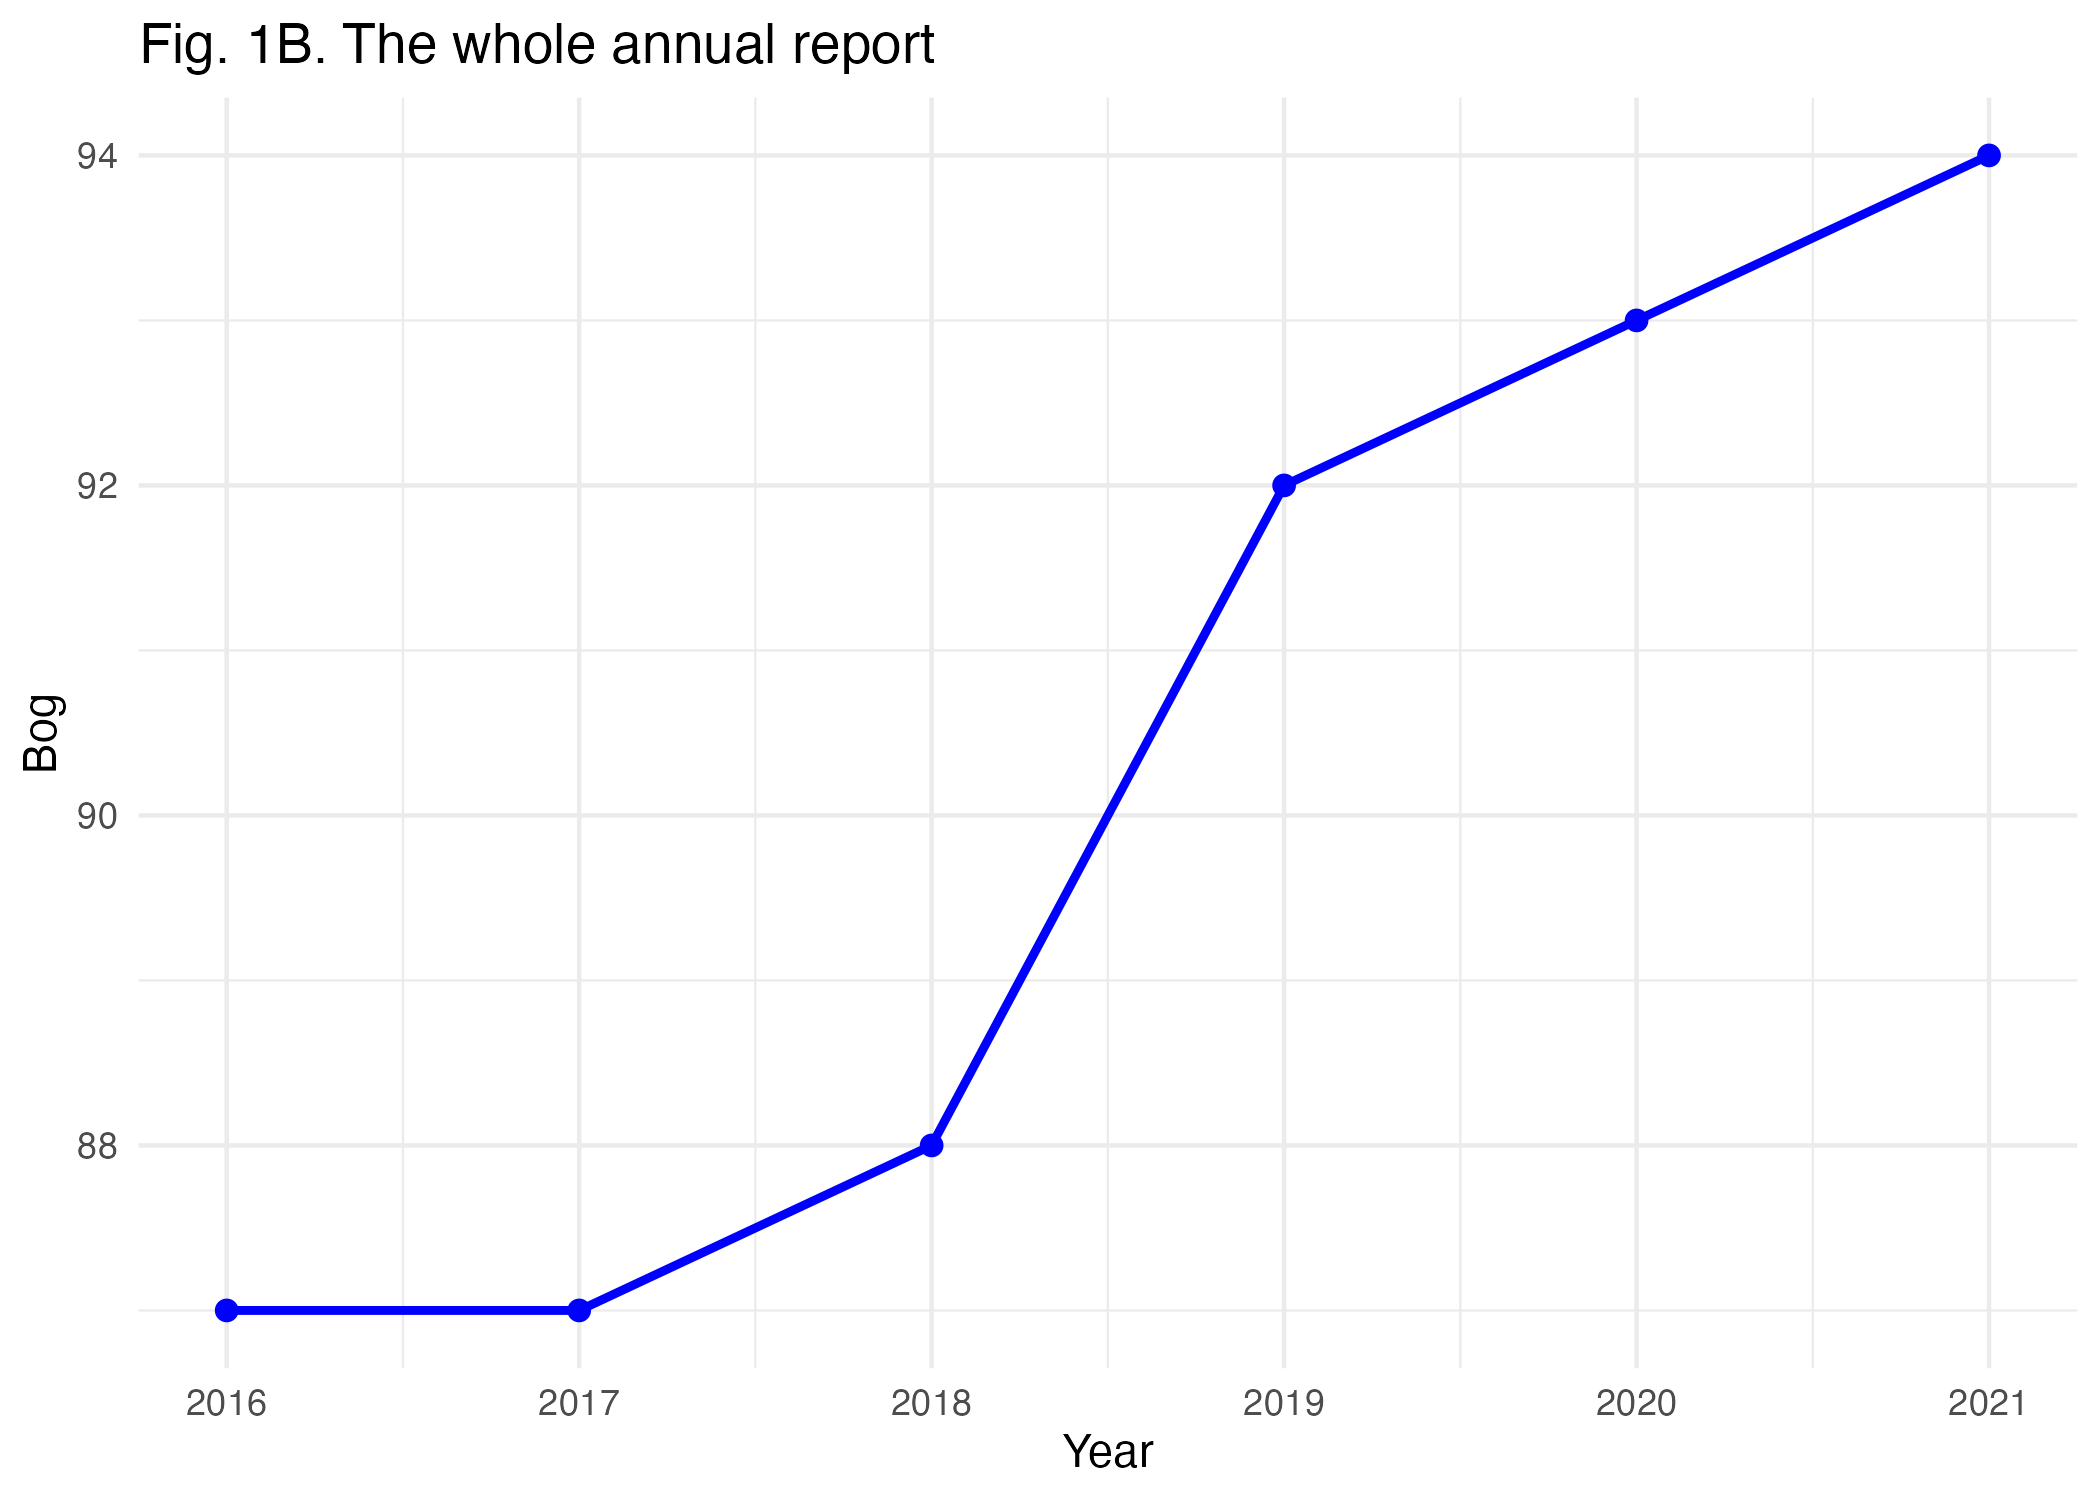
\includegraphics[width=\linewidth]{Images/fig1b.png}
\end{figure}

\begin{figure}[htbp]
    \centering
    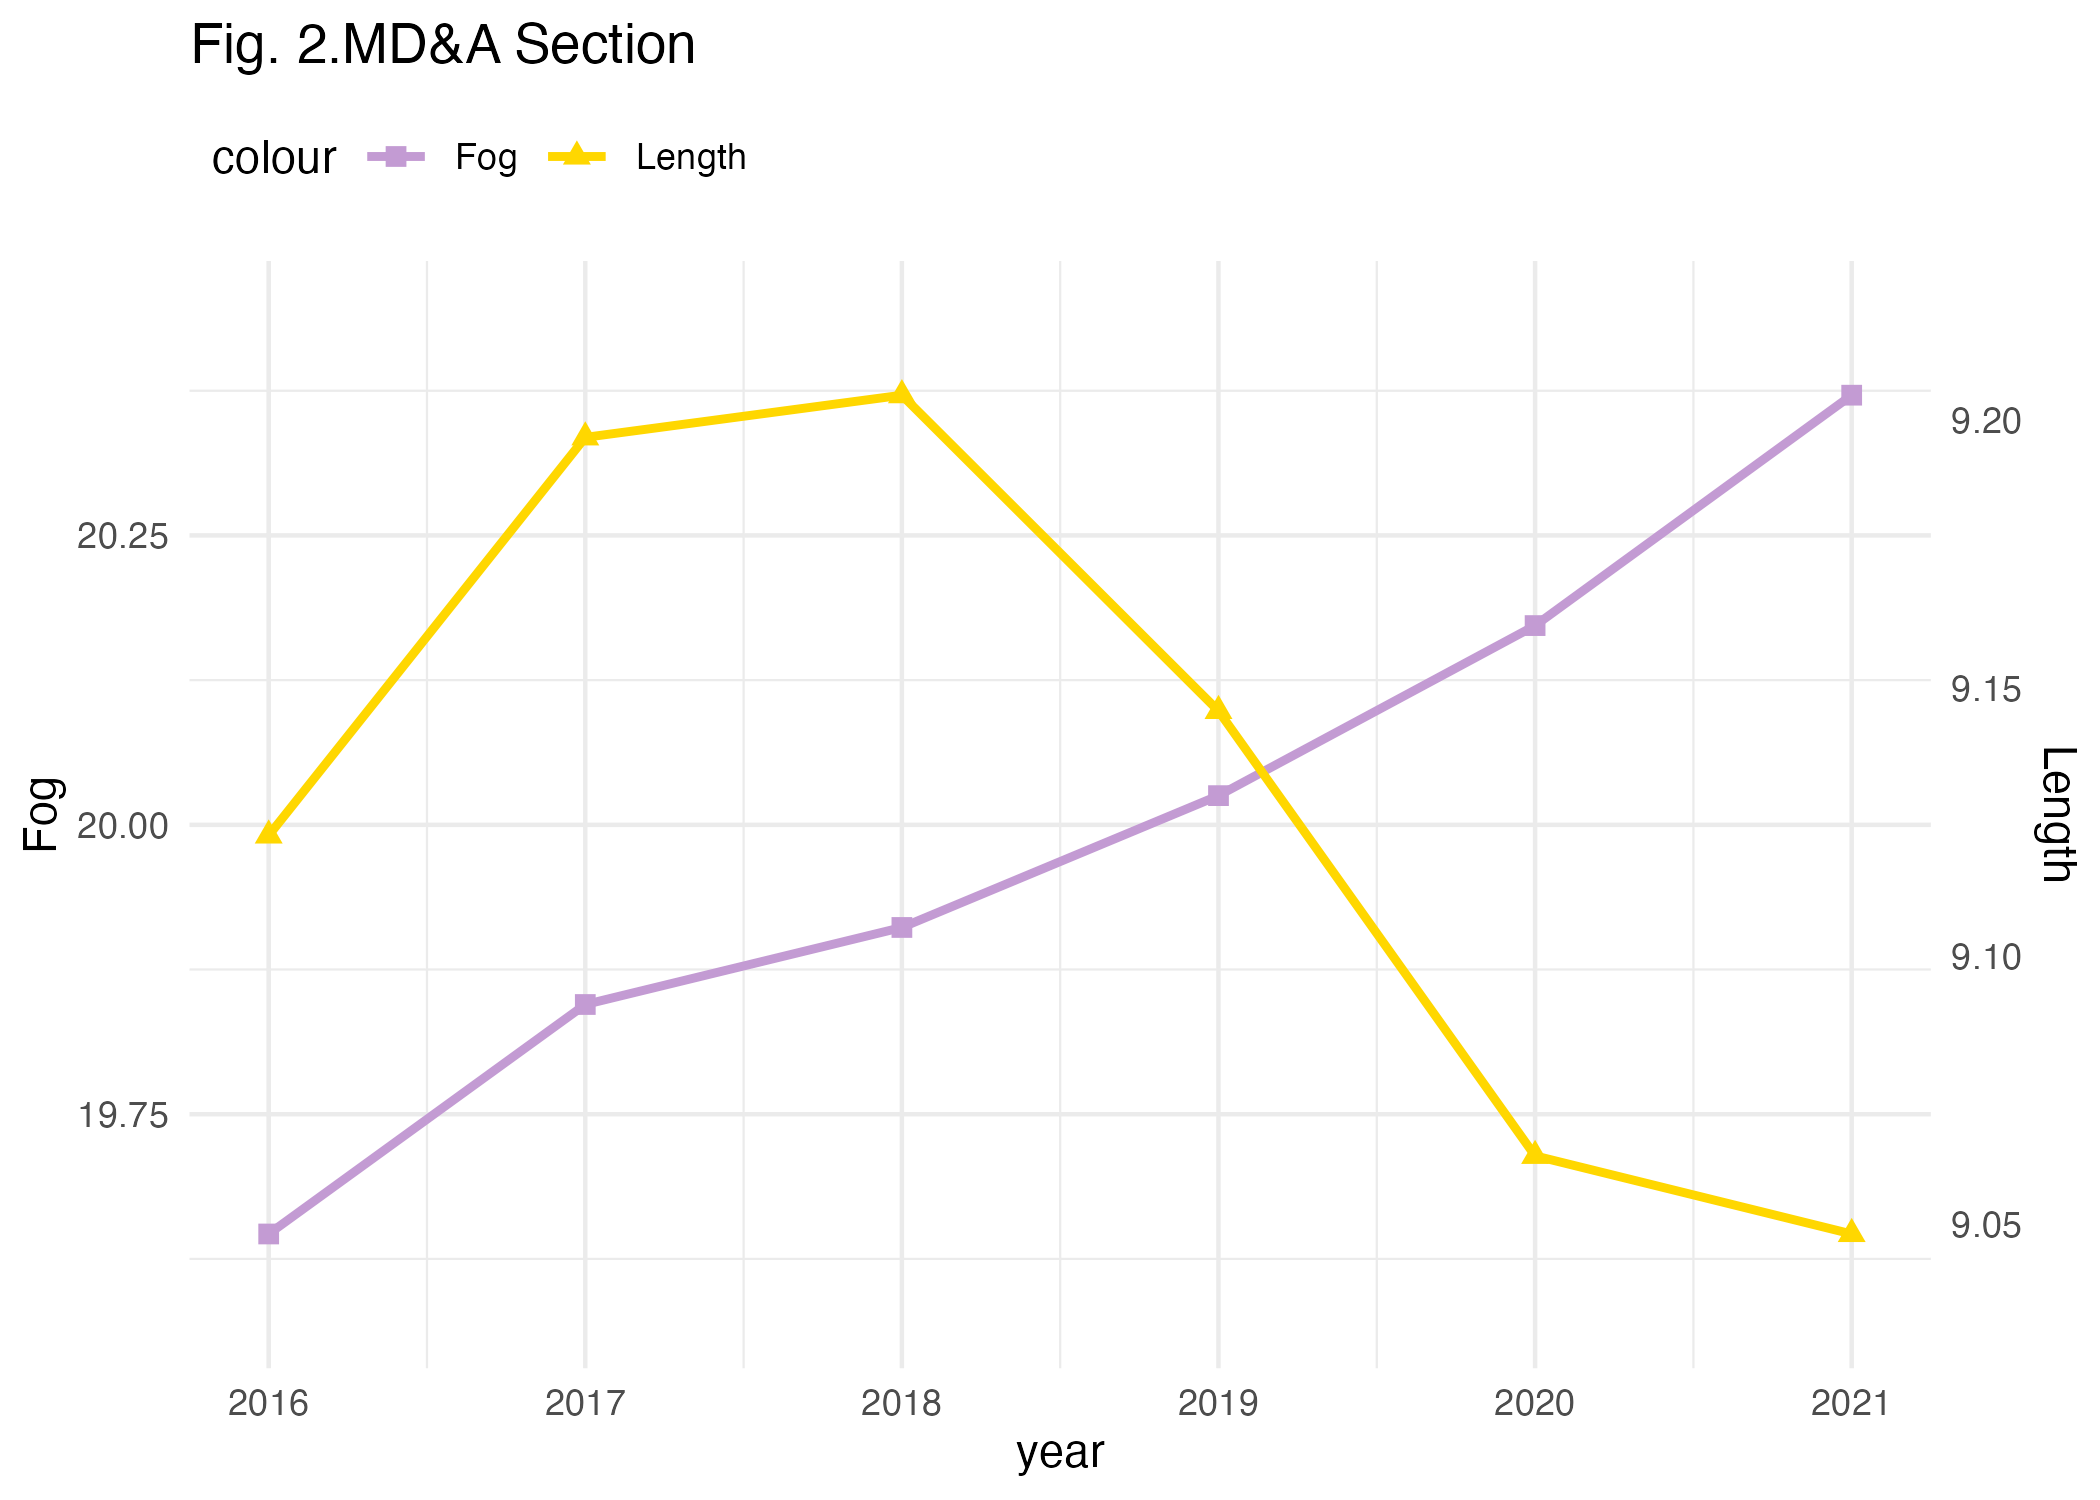
\includegraphics[width=\linewidth]{Images/fig2.png}
\end{figure}

\subsection{Determinants of Annual Report Readability}

Following Li (2008), the determinants of annual report readability are examined using the same set of firm-level control variables:

\begin{itemize} \itemsep0pt \parskip0pt \parsep0pt
\item \textit{Size}: The natural logarithm of market value of equity (data199 $\times$ data25). Larger firms are expected to produce less readable reports due to greater complexity and political costs.

\item \textit{Market-to-book}: Calculated as (market value of equity + total liabilities) divided by total assets, i.e., \((\text{data199} \times \text{data25} + \text{data181})/\text{data6}\). 

\item \textit{Firm age}: The number of years since first appearance in the CRSP monthly stock return files. Older firms are expected to issue more readable reports due to reduced information asymmetry.

\item \textit{Special items}: Special items (data17) scaled by total assets (data6). Firms with large negative special items likely experience unusual events and issue less readable disclosures.

\item \textit{Volatility}: Includes return volatility (\textit{RET\_VOL}), the standard deviation of monthly stock returns in the prior year; and earnings volatility (\textit{EARN\_VOL}), the standard deviation of operating income before depreciation (data178) scaled by assets over the past five years.

\item \textit{Operational complexity}: The log number of business segments (\textit{NBSEG}) and geographic segments (\textit{NGSEG}) from Compustat segment data. Firms with more segments are expected to report less readably.

\item \textit{Financial complexity}: The number of non-missing Compustat items (\textit{NITEMS}) for each firm-year. A greater number of reported items reflects higher reporting complexity.

\item \textit{Firm events}: Two dummies capture major events: \textit{MA} equals 1 if the firm is an acquirer in the SDC M\&A database; \textit{SEO} equals 1 if the firm issues equity in the secondary market per SDC New Issues data.

\item \textit{Incorporation state}: A Delaware dummy (\textit{DLW}) equals 1 if the firm is incorporated in Delaware, where legal and governance structures may differ.

\end{itemize}

\vspace{1em}
{\normalsize \textbf{Table 2: } \par}
{\normalsize \textbf{(A) Summary statistics of the determinants of Fog and Length;} \par}
{\normalsize \textbf{(B) Determinants of Fog; (C) Determinants of Length; (D) Determinants of Bog} \par}


\begin{subtable}[t]{\textwidth}
\centering
\begin{tabular}{lcccccc}
  \hline
 & Mean & Median & Std. Dev & 25th & 75th & N \\ 
  \hline
AGE & 20.18 & 17.00 & 18.89 & 5.00 & 28.00 & 18626 \\ 
  SI & -0.01 & -0.00 & 0.09 & -0.01 & 0.00 & 18385 \\ 
  RET\_VOL & 0.13 & 0.10 & 0.13 & 0.07 & 0.16 & 17266 \\ 
  EARN\_VOL & 0.23 & 0.04 & 3.54 & 0.02 & 0.10 & 15103 \\ 
  NBSEG & 1.63 & 1.39 & 0.60 & 1.39 & 2.20 & 17256 \\ 
  NGSEG & 1.78 & 1.61 & 0.67 & 1.39 & 2.30 & 14684 \\ 
  NITEMS & 237.64 & 247.00 & 32.27 & 237.00 & 255.00 & 18623 \\ 
  SEO & 0.02 & - & - & - & - & 18626 \\ 
  MA & 0.37 & - & - & - & - & 18626 \\ 
  DLW & 0.66 & - & - & - & - & 18626 \\ 
  \bottomrule
\end{tabular}
\end{subtable}

\vspace{1cm}

\begin{center}
\begin{longtable}{@{\extracolsep{5pt}}lcc}
\\[-1.8ex]\hline 
\hline \\[-1.8ex] 
 & \multicolumn{2}{c}{\textit{Dependent variable: Fog}} \\ 
\cline{2-3} 
\\[-1.8ex] &whole annual report&MD\&A \\ 
\\[-1.8ex] & (1) & (2)\\ 
\hline \\[-1.8ex] 
 size & 0.127$^{***}$ & 0.156$^{***}$ \\ 
  & t = 9.146 & t = 9.317 \\ 
  & & \\ 
 mtb & $-$0.045$^{***}$ & $-$0.041$^{**}$ \\ 
  & t = $-$4.955 & t = $-$2.499 \\ 
  & & \\ 
 age & $-$0.011$^{***}$ & $-$0.014$^{***}$ \\ 
  & t = $-$6.420 & t = $-$5.755 \\ 
   & & \\ 
 si & $-$0.041 & $-$0.307 \\ 
  & t = $-$0.235 & t = $-$1.445 \\ 
  & & \\ 
 RET\_VOL & 0.591$^{***}$ & 0.983$^{***}$ \\ 
  & t = 2.746 & t = 3.991 \\ 
  & & \\ 
 EARN\_VOL & 0.015$^{***}$ & 0.016$^{***}$ \\ 
  & t = 2.660 & t = 3.700 \\ 
  & & \\ 
 NBSEG & 0.003 & $-$0.025 \\ 
  & t = 0.078 & t = $-$0.373 \\ 
  & & \\ 
 NGSEG & $-$0.098 & $-$0.107 \\ 
  & t = $-$1.344 & t = $-$1.069 \\ 
  & & \\ 
 NITEMS & $-$0.00003 & 0.001 \\ 
  & t = $-$0.014 & t = 0.461 \\ 
  & & \\ 
 SEO & 0.135 & $-$0.003 \\ 
  & t = 1.483 & t = $-$0.028 \\ 
  & & \\ 
 MA & 0.034 & $-$0.005 \\ 
  & t = 0.625 & t = $-$0.092 \\ 
  & & \\ 
 DLW & 0.174$^{***}$ & 0.173$^{**}$ \\ 
  & t = 4.274 & t = 2.168 \\ 
   & & \\ 
\hline \\[-1.8ex] 
Year dummies & Yes & Yes \\ 
Industry dummies & Yes & Yes \\ 
Cluster & Sic2 & Sic2 \\ 
Observations & 12,708 & 11,968 \\ 
Adjusted R$^{2}$ & 0.132 & 0.109 \\ 
\bottomrule
\multicolumn{3}{r}{\footnotesize Note: $^{*}p<0.1$, $^{**}p<0.05$, $^{***}p<0.01$}
\end{longtable}
\end{center}
\vspace{1cm}

\begin{center}
\begin{longtable}{@{\extracolsep{5pt}}lcc}
\\[-1.8ex]\hline 
\hline \\[-1.8ex] 
 & \multicolumn{2}{c}{\textit{Dependent variable: Length}} \\ 
\cline{2-3} 
\\[-1.8ex] &whole annual report&MD\&A \\ 
\\[-1.8ex] & (1) & (2)\\ 
\hline \\[-1.8ex] 
 size & 0.091$^{***}$ & 0.174$^{***}$ \\ 
  & t = 14.556 & t = 10.319 \\ 
  & & \\ 
 mtb & $-$0.038$^{***}$ & $-$0.054$^{***}$ \\ 
  & t = $-$6.371 & t = $-$3.739 \\ 
  & & \\ 
 age & $-$0.004$^{***}$ & $-$0.011$^{***}$ \\ 
  & t = $-$6.349 & t = $-$6.254 \\ 
  & & \\ 
 si & $-$0.298$^{***}$ & $-$0.373 \\ 
  & t = $-$2.988 & t = $-$1.594 \\ 
  & & \\ 
 RET\_VOL & 0.423$^{***}$ & $-$0.057 \\ 
  & t = 4.643 & t = $-$0.220 \\ 
  & & \\ 
 EARN\_VOL & 0.004$^{*}$ & $-$0.014 \\ 
  & t = 1.734 & t = $-$0.971 \\ 
  & & \\ 
 NBSEG & 0.051$^{**}$ & 0.091$^{*}$ \\ 
  & t = 2.604 & t = 1.906 \\ 
  & & \\ 
 NGSEG & $-$0.006 & 0.080 \\ 
  & t = $-$0.266 & t = 1.304 \\ 
  & & \\ 
 NITEMS & 0.001 & 0.004 \\ 
  & t = 0.838 & t = 1.173 \\ 
  & & \\ 
 SEO & 0.061$^{***}$ & 0.148$^{**}$ \\ 
  & t = 2.765 & t = 2.123 \\ 
  & & \\ 
 MA & $-$0.006 & $-$0.060 \\ 
  & t = $-$0.427 & t = $-$1.655 \\ 
  & & \\ 
 DLW & 0.095$^{***}$ & 0.162$^{**}$ \\ 
  & t = 6.307 & t = 2.319 \\ 
  & & \\ 
\hline \\[-1.8ex] 
Year dummies & Yes & Yes \\ 
Industry dummies & Yes & Yes \\ 
Cluster & Sic2 & Sic2 \\ 
Observations & 12,708 & 12,708 \\ 
Adjusted R$^{2}$ & 0.321 & 0.084 \\ 
\hline 
\hline \\[-1.8ex] 
\textit{Note:}  & \multicolumn{2}{r}{$^{*}$p$<$0.1; $^{**}$p$<$0.05; $^{***}$p$<$0.01} \\ 
\end{longtable}
\end{center}

\begin{center}
\begin{longtable}{@{\extracolsep{5pt}}lcc}
\\[-1.8ex]\hline 
\hline \\[-1.8ex] 
 & \multicolumn{1}{c}{\textit{Dependent variable: Bog}} \\ 
\cline{2-2} 
\\[-1.8ex] & whole annual report \\ 
\hline \\[-1.8ex] 
 size & 1.040$^{***}$ \\ 
  & t = 8.393 \\ 
  & \\ 
 mtb & $-$0.347$^{**}$ \\ 
  & t = $-$2.431 \\ 
  & \\ 
 age & $-$0.049$^{***}$ \\ 
  & t = $-$4.023 \\ 
  & \\ 
 si & $-$2.480$^{***}$ \\ 
  & t = $-$2.843 \\ 
  & \\ 
 RET\_VOL & 2.361$^{**}$ \\ 
  & t = 2.131 \\ 
  & \\ 
 EARN\_VOL & 0.064$^{*}$ \\ 
  & t = 1.945 \\ 
  & \\ 
 NBSEG & 0.532 \\ 
  & t = 1.264 \\ 
  & \\ 
 NGSEG & $-$0.618 \\ 
  & t = $-$0.928 \\ 
  & \\ 
 NITEMS & $-$0.002 \\ 
  & t = $-$0.076 \\ 
  & \\ 
 SEO & 0.349 \\ 
  & t = 0.653 \\ 
  & \\ 
 MA & $-$0.581 \\ 
  & t = $-$1.471 \\ 
  & \\ 
 DLW & 1.628$^{***}$ \\ 
  & t = 3.861 \\ 
  & \\ 
\hline \\[-1.8ex] 
Year dummies & Yes \\ 
Industry dummies & Yes \\ 
Cluster & Sic2 \\ 
Observations & 12,708 \\ 
Adjusted R$^{2}$ & 0.341 \\ 
\hline 
\hline \\[-1.8ex] 
\textit{Note:}  & \multicolumn{1}{r}{$^{*}$p$<$0.1; $^{**}$p$<$0.05; $^{***}$p$<$0.01} \\ 

\end{longtable}
\end{center}

Table~2 presents the results of regressing the Fog, Length and Bog indices on their potential determinants, with standard errors clustered at the two-digit SIC level. All models include year and industry fixed effects.

Panel~A summarizes firm-level control variables. Panel~B of Table~2 investigates determinants of the Fog index for both the entire annual report and the MD\&A section. Column~(1) indicates that larger firms, firms with higher return volatility, greater earnings volatility, and Delaware incorporation are associated with more complex disclosures. Conversely, \textit{MTB} and \textit{AGE} exhibit negative and statistically significant coefficients ($\beta = -0.045$, $t = -4.96$; $\beta = -0.011$, $t = -6.42$), indicating that older and higher-valued firms tend to produce more readable reports. Column~(2) shows similar associations for the MD\&A section, with \textit{SIZE}, \textit{RET\_VOL}, \textit{EARN\_VOL}, and \textit{DLW} remaining positively associated with Fog, and \textit{AGE} and \textit{MTB} maintaining negative signs. The adjusted $R^2$ values are 0.132 and 0.109 for the full report and MD\&A, respectively, suggesting moderate explanatory power.

Panel~C examines the determinants of disclosure length. In column~(1), length of the whole annual report is strongly associated with firm size ($\beta = 0.091$), Delaware-incorporated firms ($\beta = 0.095$), firms issuing secondary equity ($\beta = 0.061$)and those with more business segments ($\beta = 0.051$). As in Panel~B, \textit{AGE} and \textit{MTB} are negatively associated with disclosure length, although the estimated effects are relatively modest. The adjusted $R^2$ of 0.321 indicates that firm characteristics explain a substantially larger share of variation in disclosure length than in textual complexity. For the MD\&A section (column~2), firm size, Delaware incorporation, and secondary equity offerings remain statistically significant predictors of disclosure length. In contrast, volatility measures lose explanatory power in this specification. The adjusted $R^2$ of 0.084 suggests limited explanatory power for MD\&A length.

Panel~D assesses the determinants of the Bog Index, which captures deviations from plain English writing standards. Firm size and Delaware incorporation are strongly associated with more linguistically complex language. Volatile firms—measured by return volatility ($\beta = 2.361$, $t = 2.13$) and earnings volatility ($\beta = 0.064$, $t = 1.95$)—also display significantly lower adherence to plain English. In contrast, older firms and those with higher market-to-book ratios are more compliant with plain language conventions. Special items are negatively associated with the Bog Index ($\beta = -2.480$, $t = -2.84$), potentially reflecting strategic clarity in explaining extraordinary items. The model explains a relatively large share of the variation in Bog scores, with an adjusted $R^2$ of 0.341.

\section{Analysis and results}
\subsection{Current earnings and annual report readability}

{\normalsize \textbf{Table 3: } \par}
{\normalsize \textbf{(A) Firm performance and annual report Fog and Length (level specification); } \par}
{\normalsize \textbf{(B) Firm performance and annual report Fog and Length (change specification)} \par}

\begin{tabular}{@{\extracolsep{5pt}}lcccccc} 
\\[-1.8ex]\hline 
\hline \\[-1.8ex] 
 & \multicolumn{6}{c}{\textit{Whole annual report Dependent variable:}} \\ 
\cline{2-7} 
\\[-1.8ex] & \multicolumn{2}{c}{Fog} & \multicolumn{2}{c}{Length} & \multicolumn{2}{c}{Bog} \\ 
\\[-1.8ex] & (1) & (2) & (3) & (4) & (5) & (6)\\ 
\hline \\[-1.8ex] 
 Earnings & $-$1.032$^{***}$ &  & $-$0.503$^{***}$ &  & $-$6.753$^{***}$ &  \\ 
  & t = $-$5.676 &  & t = $-$12.463 &  & t = $-$2.835 &  \\ 
  & & & & & & \\ 
 Profit/loss &  & $-$0.342$^{***}$ &  & $-$0.175$^{***}$ &  & $-$2.154$^{*}$ \\ 
  &  & t = $-$3.359 &  & t = $-$4.961 &  & t = $-$1.766 \\ 
  & & & & & & \\ 
\hline \\[-1.8ex] 
Year dummies & Yes & Yes & Yes & Yes & Yes & Yes \\ 
Industry dummies & Yes & Yes & Yes & Yes & Yes & Yes \\ 
Control variables & Yes & Yes & Yes & Yes & Yes & Yes \\ 
Cluster & Sic2 & Sic2 & Sic2 & Sic2 & Sic2 & Sic2 \\ 
Observations & 12,708 & 12,708 & 12,708 & 12,708 & 12,708 & 12,708 \\ 
Adjusted R$^{2}$ & 0.146 & 0.140 & 0.350 & 0.340 & 0.355 & 0.349 \\ 
\hline 
\hline \\[-1.8ex] 
\textit{Note:}  & \multicolumn{6}{r}{$^{*}$p$<$0.1; $^{**}$p$<$0.05; $^{***}$p$<$0.01} \\ 
\end{tabular} 

\begin{center}
\begin{longtable}{@{\extracolsep{5pt}}lcccc} 
\\[-1.8ex]\hline 
\hline \\[-1.8ex] 
 & \multicolumn{4}{c}{\textit{MD\&A Section Dependent variable:}} \\ 
\cline{2-5} 
\\[-1.8ex] & \multicolumn{2}{c}{Fog} & \multicolumn{2}{c}{Length} \\ 
\\[-1.8ex] & (1) & (2) & (3) & (4)\\ 
\hline \\[-1.8ex] 
 Earnings & $-$1.459$^{***}$ &  & 0.045 &  \\ 
  & t = $-$6.507 &  & t = 0.303 &  \\ 
  & & & & \\ 
 Profit/loss &  & $-$0.480$^{***}$ &  & 0.041 \\ 
  &  & t = $-$3.593 &  & t = 0.490 \\ 
  & & & & \\ 
\hline \\[-1.8ex] 
Year dummies & Yes & Yes & Yes & Yes \\ 
Industry dummies & Yes & Yes & Yes & Yes \\ 
Control variables & Yes & Yes & Yes & Yes \\ 
Cluster & Sic2 & Sic2 & Sic2 & Sic2 \\ 
Observations & 11,968 & 11,968 & 12,708 & 12,708 \\ 
Adjusted R$^{2}$ & 0.123 & 0.117 & 0.084 & 0.084 \\ 
\hline 
\hline \\[-1.8ex] 
\textit{Note:}  & \multicolumn{4}{r}{$^{*}$p$<$0.1; $^{**}$p$<$0.05; $^{***}$p$<$0.01} \\ 
\end{longtable}
\end{center}
 
\begin{center}
\begin{longtable}{@{\extracolsep{5pt}}lcccccc} 
\\[-1.8ex]\hline 
\hline \\[-1.8ex] 
 & \multicolumn{6}{c}{\textit{Whole annual report Dependent variable:}} \\ 
\cline{2-7} 
\\[-1.8ex] & \multicolumn{2}{c}{\(\Delta\)Fog} & \multicolumn{2}{c}{\(\Delta\)Length} & \multicolumn{2}{c}{\(\Delta\)Bog} \\ 
\\[-1.8ex] & (1) & (2) & (3) & (4) & (5) & (6)\\ 
\hline \\[-1.8ex] 
 Change in earnings & $-$0.067 &  & $-$0.059$^{*}$ &  & $-$0.480 &  \\ 
  & t = $-$0.557 &  & t = $-$1.979 &  & t = $-$0.751 &  \\ 
  & & & & & & \\ 
 Earnings \(\pm\) \text{Dummy} &  & $-$0.009 &  & $-$0.016$^{**}$ &  & $-$0.141 \\ 
  &  & t = $-$0.318 &  & t = $-$2.290 &  & t = $-$1.134 \\ 
  & & & & & & \\ 
\hline \\[-1.8ex] 
Year dummies & Yes & Yes & Yes & Yes & Yes & Yes \\ 
Industry dummies & Yes & Yes & Yes & Yes & Yes & Yes \\ 
Control variables & Yes & Yes & Yes & Yes & Yes & Yes \\ 
Cluster & Sic2 & Sic2 & Sic2 & Sic2 & Sic2 & Sic2 \\ 
Observations & 10,844 & 10,844 & 10,844 & 10,844 & 10,844 & 10,844 \\ 
Adjusted R$^{2}$ & $-$0.001 & $-$0.001 & 0.005 & 0.005 & 0.055 & 0.055 \\ 
\hline 
\hline \\[-1.8ex] 
\textit{Note:}  & \multicolumn{6}{r}{$^{*}$p$<$0.1; $^{**}$p$<$0.05; $^{***}$p$<$0.01} \\ 

\end{longtable}
\end{center}


\begin{center}
\begin{longtable}{@{\extracolsep{5pt}}lcccc} 
\\[-1.8ex]\hline 
\hline \\[-1.8ex] 
 & \multicolumn{4}{c}{\textit{MD\&A Section Dependent variable:}} \\ 
\cline{2-5} 
\\[-1.8ex] & \multicolumn{2}{c}{\(\Delta\)Fog} & \multicolumn{2}{c}{\(\Delta\)Length} \\ 
\\[-1.8ex] & (1) & (2) & (3) & (4)\\ 
\hline \\[-1.8ex] 
 Change in earnings & $-$0.186$^{*}$ &  & 0.091 &  \\ 
  & t = $-$1.846 &  & t = 0.504 &  \\ 
  & & & & \\ 
 Earnings \(\pm\) \text{Dummy} &  & $-$0.028 &  & $-$0.029 \\ 
  &  & t = $-$1.351 &  & t = $-$0.873 \\ 
  & & & & \\ 
\hline \\[-1.8ex] 
Year dummies & Yes & Yes & Yes & Yes \\ 
Industry dummies & Yes & Yes & Yes & Yes \\ 
Control variables & Yes & Yes & Yes & Yes \\ 
Cluster & Sic2 & Sic2 & Sic2 & Sic2 \\ 
Observations & 10,019 & 10,019 & 10,844 & 10,844 \\ 
Adjusted R$^{2}$ & $-$0.001 & $-$0.001 & 0.013 & 0.013 \\ 
\hline 
\hline \\[-1.8ex] 
\textit{Note:}  & \multicolumn{4}{r}{$^{*}$p$<$0.1; $^{**}$p$<$0.05; $^{***}$p$<$0.01} \\ 
\end{longtable}
\end{center}

Table 3 presents the results of regressing the Fog and Length on earnings (scaled by book value of assets) using both level specification (Panel A) and change specification (Panel B). 

In columns~(1), (3), and (5) of Panel~A (Whole Annual Report), higher earnings are significantly associated with more readable disclosures, as evidenced by negative coefficients on the Fog ($\beta = -1.032$, $t = -5.68$), Length ($\beta = -0.503$, $t = -12.46$), and Bog indices ($\beta = -6.753$, $t = -2.84$). Similarly, firms reporting positive earnings (captured by the profit dummy) also produce clearer disclosures: $\beta = -0.342$ ($t = -3.36$) for Fog, $\beta = -0.175$ ($t = -4.96$) for Length, and $\beta = -2.154$ ($t = -1.77$) for the Bog index. These findings align with prior literature that the annual reports of loss firms are more difficult to read than those of profit firms. The MD&A section results (bottom of Panel~A) show a consistent pattern, with earnings negatively correlated with MD&A Fog ($\beta = -1.459$, $t = -6.51$), although the association with length is insignificant.

Panel~B presents change specifications, analyzing year-over-year changes in Fog, Bog, and Length indices. Results here are weaker. Earnings changes are negatively but insignificantly associated with changes in Fog and Bog, and only marginally significantly with changes in report length ($\beta = -0.059$, $t = -1.98$). For the MD&A section, earnings changes negatively associate with Fog changes ($\beta = -0.186$, $t = -1.85$) but are insignificant for length changes. The low adjusted \( R^2 \) across the change regressions suggests that much of the variation in disclosure readability remains unexplained in a first-difference specification.


\subsection{Earnings Persistence and Annual Report Readability}


{\normalsize \textbf{Table 4: } \par}
{\normalsize \textbf{(A) Earnings persistence and annual report Fog index (profit firm-years);} \par}
{\normalsize \textbf{(B) Earnings persistence and annual report Length (profit firm-years);} \par}
{\normalsize \textbf{(C) Earnings persistence and annual report Bog (profit firm-years);} \par}
{\normalsize \textbf{(D) Earnings persistence and annual report readability (profit firm-years);} \par}

\begin{tabular}{@{\extracolsep{5pt}}lcccc} 
\\[-1.8ex]\hline 
\hline \\[-1.8ex] 
 & \multicolumn{4}{c}{\textit{Dependent variable:}} \\ 
\cline{2-5} 
\\[-1.8ex] & \(\text{Earn}(t{+}1)\) & \(\text{Earn}(t{+}2)\) & \(\text{Earn}(t{+}1)\) & \(\text{Earn}(t{+}2)\) \\ 
\\[-1.8ex] & (1) & (2) & (3) & (4)\\ 
\hline \\[-1.8ex] 
 Earnings & 1.592$^{***}$ & 1.731$^{***}$ & 1.560$^{***}$ & 1.530$^{***}$ \\ 
  & t = 3.620 & t = 3.154 & t = 3.236 & t = 2.797 \\ 
  & & & & \\ 
 fog\_index & 0.002 & 0.003 &  &  \\ 
  & t = 1.573 & t = 1.569 &  &  \\ 
  & & & & \\ 
 mda\_fog\_index &  &  & 0.003 & 0.003 \\ 
  &  &  & t = 1.555 & t = 1.253 \\ 
  & & & & \\ 
 Earnings:fog\_index & $-$0.043$^{*}$ & $-$0.058$^{*}$ &  &  \\ 
  & t = $-$1.789 & t = $-$1.927 &  &  \\ 
  & & & & \\ 
 Earnings:mda\_fog\_index &  &  & $-$0.042 & $-$0.049 \\ 
  &  &  & t = $-$1.566 & t = $-$1.584 \\ 
  & & & & \\ 
\hline \\[-1.8ex] 
Year dummies & Yes & Yes & Yes & Yes \\ 
Industry dummies & Yes & Yes & Yes & Yes \\ 
Control variables & Yes & Yes & Yes & Yes \\ 
Cluster & Sic2 & Sic2 & Sic2 & Sic2 \\ 
Observations & 7,818 & 6,445 & 7,487 & 6,218 \\ 
Adjusted R$^{2}$ & 0.525 & 0.396 & 0.548 & 0.403 \\ 
\hline 
\hline \\[-1.8ex] 
\textit{Note:}  & \multicolumn{4}{r}{$^{*}$p$<$0.1; $^{**}$p$<$0.05; $^{***}$p$<$0.01} \\ 
\end{tabular} 
\end{table} 

\begin{center}
\begin{longtable}{@{\extracolsep{5pt}}lcccc} 
\\[-1.8ex]\hline 
\hline \\[-1.8ex] 
 & \multicolumn{4}{c}{\textit{Dependent variable:}} \\ 
\cline{2-5} 
\\[-1.8ex] & \(\text{Earn}(t{+}1)\) & \(\text{Earn}(t{+}2)\) & \(\text{Earn}(t{+}1)\) & \(\text{Earn}(t{+}2)\) \\ 
\\[-1.8ex] & (1) & (2) & (3) & (4)\\ 
\hline \\[-1.8ex] 
 Earnings & 2.919$^{**}$ & 2.930$^{**}$ & 0.570$^{***}$ & 0.442$^{***}$ \\ 
  & t = 2.594 & t = 2.161 & t = 7.108 & t = 3.867 \\ 
  & & & & \\ 
 length & 0.009 & 0.008 &  &  \\ 
  & t = 1.537 & t = 0.968 &  &  \\ 
  & & & & \\ 
 mda\_length &  &  & $-$0.0005 & $-$0.001 \\ 
  &  &  & t = $-$0.847 & t = $-$0.611 \\ 
  & & & & \\ 
 Earnings:length & $-$0.203$^{*}$ & $-$0.220$^{*}$ &  &  \\ 
  & t = $-$1.878 & t = $-$1.693 &  &  \\ 
  & & & & \\ 
 Earnings:mda\_length &  &  & 0.016$^{***}$ & 0.012 \\ 
  &  &  & t = 3.283 & t = 0.801 \\ 
  & & & & \\ 
\hline \\[-1.8ex] 
Year dummies & Yes & Yes & Yes & Yes \\ 
Industry dummies & Yes & Yes & Yes & Yes \\ 
Control variables & Yes & Yes & Yes & Yes \\ 
Cluster & Sic2 & Sic2 & Sic2 & Sic2 \\ 
Observations & 7,818 & 6,445 & 7,818 & 6,445 \\ 
Adjusted R$^{2}$ & 0.529 & 0.399 & 0.523 & 0.391 \\ 
\hline 
\hline \\[-1.8ex] 
\textit{Note:}  & \multicolumn{4}{r}{$^{*}$p$<$0.1; $^{**}$p$<$0.05; $^{***}$p$<$0.01} \\ 
\end{longtable}
\end{center}

\begin{center}
\begin{longtable}{@{\extracolsep{5pt}}lcc} 
\\[-1.8ex]\hline 
\hline \\[-1.8ex] 
 & \multicolumn{2}{c}{\textit{Dependent variable:}} \\ 
\cline{2-3} 
\\[-1.8ex] & \(\text{Earn}(t{+}1)\) & \(\text{Earn}(t{+}2)\) \\ 
\\[-1.8ex] & (1) & (2)\\ 
\hline \\[-1.8ex] 
 Earnings & 1.587$^{***}$ & 1.660$^{***}$ \\ 
  & t = 4.901 & t = 4.330 \\ 
  & & \\ 
 bogindex & 0.0005$^{*}$ & 0.001$^{**}$ \\ 
  & t = 1.884 & t = 2.206 \\ 
  & & \\ 
 Earnings:bogindex & $-$0.010$^{**}$ & $-$0.013$^{**}$ \\ 
  & t = $-$2.347 & t = $-$2.549 \\ 
  & & \\ 
\hline \\[-1.8ex] 
Year dummies & Yes & Yes \\ 
Industry dummies & Yes & Yes \\ 
Control variables & Yes & Yes \\ 
Cluster & Sic2 & Sic2 \\ 
Observations & 7,818 & 6,445 \\ 
Adjusted R$^{2}$ & 0.528 & 0.399 \\ 
\hline 
\hline \\[-1.8ex] 
\textit{Note:}  & \multicolumn{2}{r}{$^{*}$p$<$0.1; $^{**}$p$<$0.05; $^{***}$p$<$0.01} \\ 
\end{longtable}
\end{center}

\begin{center} 
\begin{longtable}{@{\extracolsep{5pt}}lcccc} 
\\[-1.8ex]\hline 
\hline \\[-1.8ex] 
 & \multicolumn{4}{c}{\textit{Dependent variable:}} \\ 
\cline{2-5} 
\\[-1.8ex] & \(\text{Earn}(t{+}1)\) & \(\text{Earn}(t{+}2)\) & \(\text{Earn}(t{+}1)\) & \(\text{Earn}(t{+}2)\) \\ 
\\[-1.8ex] & (1) & (2) & (3) & (4)\\ 
\hline \\[-1.8ex] 
 Earnings & 1.893$^{***}$ & 2.008$^{***}$ & 2.942$^{**}$ & 2.965$^{**}$ \\ 
  & t = 3.040 & t = 2.860 & t = 2.607 & t = 2.212 \\ 
  & & & & \\ 
 fog\_index & 0.001$^{*}$ & 0.002$^{*}$ &  &  \\ 
  & t = 1.716 & t = 1.940 &  &  \\ 
  & & & & \\ 
 mda\_fog\_index & 0.002 & 0.002 &  &  \\ 
  & t = 1.475 & t = 1.071 &  &  \\ 
  & & & & \\ 
 length &  &  & 0.011$^{*}$ & 0.010 \\ 
  &  &  & t = 1.698 & t = 1.261 \\ 
  & & & & \\ 
 mda\_length &  &  & $-$0.001 & $-$0.002 \\ 
  &  &  & t = $-$1.577 & t = $-$1.480 \\ 
  & & & & \\ 
 Earnings:fog\_index & $-$0.026$^{*}$ & $-$0.036$^{**}$ &  &  \\ 
& t = $-$1.866 & t = $-$2.296 &  &  \\ 
  & & & & \\ 
 Earnings:mda\_fog\_index & $-$0.032 & $-$0.036 &  &  \\ 
  & t = $-$1.454 & t = $-$1.391 &  &  \\ 
  & & & & \\ 
 Earnings:length &  &  & $-$0.229$^{**}$ & $-$0.246$^{*}$ \\ 
  &  &  & t = $-$2.013 & t = $-$1.914 \\ 
  & & & & \\ 
 Earnings:mda\_length &  &  & 0.030$^{***}$ & 0.029$^{**}$ \\ 
  &  &  & t = 3.170 & t = 2.010 \\ 
  & & & & \\ 
\hline \\[-1.8ex] 
Year dummies & Yes & Yes & Yes & Yes \\ 
Industry dummies & Yes & Yes & Yes & Yes \\ 
Control variables & Yes & Yes & Yes & Yes \\ 
Cluster & Sic2 & Sic2 & Sic2 & Sic2 \\ 
Observations & 7,487 & 6,218 & 7,818 & 6,445 \\ 
Adjusted R$^{2}$ & 0.549 & 0.405 & 0.531 & 0.400 \\ 
\hline 
\hline \\[-1.8ex] 
\textit{Note:}  & \multicolumn{4}{r}{$^{*}$p$<$0.1; $^{**}$p$<$0.05; $^{***}$p$<$0.01} \\ 
\end{longtable}
\end{center}

Table~4 examines the association between annual report readability and earnings persistence among profit firm-years. Following prior literature, future earnings in year $t+1$ and $t+2$ are regressed on current earnings, various readability metrics (Fog, Length, and Bog), and their interactions with current earnings. All regressions control for year and industry fixed effects, as well as standard firm-level covariates, with standard errors clustered at the two-digit SIC level.

Across Panels~A–C, current earnings are positively and significantly associated with future earnings, consistent with strong earnings persistence. Notably, the interaction terms between current earnings and each readability measure of the full annual report are negative and statistically significant. Specifically, higher Fog scores are associated with reduced earnings persistence ($\beta = -0.043$, $t = -1.79$ for $t+1$; $\beta = -0.058$, $t = -1.93$ for $t+2$), as are longer disclosures ($\beta = -0.203$, $t = -1.88$; $\beta = -0.220$, $t = -1.69$) and higher Bog scores ($\beta = -0.010$, $t = -2.35$; $\beta = -0.013$, $t = -2.55$). These results suggest that greater textual complexity and deviation from plain English weaken the information content of current earnings with respect to future performance.

Panel~D considers all readability measures. The interaction terms for Fog and Length of the full annual report remain negative and statistically significant, reinforcing prior results. In particular, the earnings–Fog interaction yields $\beta = -0.036$ ($t = -2.30$) and the earnings–Length interaction yields $\beta = -0.246$ ($t = -1.91$) in predicting $t+2$ earnings. Notably, the MD\&A length interaction is positive and significant ($\beta = 0.030$, $t = 3.17$), highlighting the incremental informativeness of narrative disclosures in that section.


{\normalsize \textbf{Table 5: } \par}
{\normalsize \textbf{(A) Earnings persistence and annual report Fog index (loss firm-years);} \par}
{\normalsize \textbf{(B) Earnings persistence and annual report Length (loss firm-years);} \par}

\begin{tabular}{@{\extracolsep{5pt}}lcccc} 
\\[-1.8ex]\hline 
\hline \\[-1.8ex] 
 & \multicolumn{4}{c}{\textit{Dependent variable:}} \\ 
\cline{2-5} 
\\[-1.8ex] & \(\text{Earn}(t{+}1)\) & \(\text{Earn}(t{+}2)\) & \(\text{Earn}(t{+}1)\) & \(\text{Earn}(t{+}2)\) \\ 
\\[-1.8ex] & (1) & (2) & (3) & (4)\\ 
\hline \\[-1.8ex] 
 Earnings & 1.210$^{***}$ & 0.920$^{*}$ & 0.582$^{*}$ & 0.368 \\ 
  & t = 3.191 & t = 1.834 & t = 1.886 & t = 0.925 \\ 
  & & & & \\ 
 fog\_index & $-$0.007 & $-$0.011$^{**}$ &  &  \\ 
  & t = $-$1.262 & t = $-$2.330 &  &  \\ 
  & & & & \\ 
 mda\_fog\_index &  &  & $-$0.004 & $-$0.003 \\ 
  &  &  & t = $-$1.244 & t = $-$0.812 \\ 
  & & & & \\ 
 Earnings:fog\_index & $-$0.029 & $-$0.023 &  &  \\ 
  & t = $-$1.667 & t = $-$1.109 &  &  \\ 
  & & & & \\ 
 Earnings:mda\_fog\_index &  &  & 0.001 & 0.003 \\ 
  &  &  & t = 0.087 & t = 0.182 \\ 
  & & & & \\ 
  \hline \\[-1.8ex] 
Year dummies & Yes & Yes & Yes & Yes \\ 
Industry dummies & Yes & Yes & Yes & Yes \\ 
Control variables & Yes & Yes & Yes & Yes \\ 
Cluster & Sic2 & Sic2 & Sic2 & Sic2 \\ 
Observations & 2,643 & 2,039 & 2,476 & 1,940 \\ 
Adjusted R$^{2}$ & 0.533 & 0.437 & 0.535 & 0.438 \\ 
\hline 
\hline \\[-1.8ex] 
\textit{Note:}  & \multicolumn{4}{r}{$^{*}$p$<$0.1; $^{**}$p$<$0.05; $^{***}$p$<$0.01} \\ 
\end{tabular} 
\end{table}

\begin{center}
\begin{longtable}{@{\extracolsep{5pt}}lcccc} 
\\[-1.8ex]\hline 
\hline \\[-1.8ex] 
 & \multicolumn{4}{c}{\textit{Dependent variable:}} \\ 
\cline{2-5} 
\\[-1.8ex] & \(\text{Earn}(t{+}1)\) & \(\text{Earn}(t{+}2)\) & \(\text{Earn}(t{+}1)\) & \(\text{Earn}(t{+}2)\) \\ 
\\[-1.8ex] & (1) & (2) & (3) & (4)\\ 
\hline \\[-1.8ex] 
 Earnings & 1.586$^{***}$ & 1.422 & 0.630$^{***}$ & 0.500$^{***}$ \\ 
  & t = 3.293 & t = 1.532 & t = 14.611 & t = 5.819 \\ 
  & & & & \\ 
 length & $-$0.020$^{*}$ & $-$0.022 &  &  \\ 
  & t = $-$1.753 & t = $-$1.368 &  &  \\ 
  & & & & \\ 
 mda\_length &  &  & 0.001 & 0.001 \\ 
  &  &  & t = 0.721 & t = 0.155 \\ 
  & & & & \\ 
 Earnings:length & $-$0.088$^{*}$ & $-$0.089 &  &  \\ 
  & t = $-$1.954 & t = $-$1.066 &  &  \\ 
  & & & & \\ 
 Earnings:mda\_length &  &  & $-$0.002 & $-$0.008 \\ 
  &  &  & t = $-$0.349 & t = $-$0.720 \\ 
  & & & & \\ 
  \hline \\[-1.8ex] 
Year dummies & Yes & Yes & Yes & Yes \\ 
Industry dummies & Yes & Yes & Yes & Yes \\ 
Control variables & Yes & Yes & Yes & Yes \\ 
Cluster & Sic2 & Sic2 & Sic2 & Sic2 \\ 
Observations & 2,643 & 2,039 & 2,643 & 2,039 \\ 
Adjusted R$^{2}$ & 0.533 & 0.437 & 0.532 & 0.436 \\ 
\hline 
\hline \\[-1.8ex] 
\textit{Note:}  & \multicolumn{4}{r}{$^{*}$p$<$0.1; $^{**}$p$<$0.05; $^{***}$p$<$0.01} \\ 
\end{longtable}
\end{center}

Although the coefficients on \textit{fog\_index} and \textit{length} in predicting future earnings at both $t{+}1$ and $t{+}2$ are slightly larger than those reported in Li~(2008), they remain statistically insignificant and economically modest. Similarly, the interaction terms between earnings and \textit{fog\_index} exhibit limited magnitude and lack statistical significance. Evidence from \textit{length} (Panel~B) aligns with this pattern, with the exception that the length of the full annual report is negatively associated with earnings persistence at the two-year horizon, suggesting only marginal explanatory power. Overall, these results provide limited evidence that annual report readability meaningfully influences the persistence of losses, consistent with the conclusions in the replicated study.

\section{Conclusion}

This study replicates Li (2008) using data from 2016–2021 and confirms a robust relationship between annual report readability and earnings outcomes. Firms with weaker performance tend to issue less readable disclosures—characterized by longer reports and higher Fog and Bog Index scores—consistent with the idea that complexity is used to obscure bad news. Conversely, firms producing clearer reports exhibit more persistent positive earnings. These findings closely align with those of the original study and are further reinforced by the inclusion of the Bog Index, which captures a broader set of plain English attributes.

This study does come with limitations. In particular, first-difference models show low explanatory power, suggesting that readability alone does not account for changes in earnings persistence. Moreover, the increasing use of AI-generated disclosures introduces new challenges for measuring readability and understanding how such automation may influence stakeholder interpretation.

 
\bibliographystyle{unsrt}
\bibliography{thesis}
\end{document}